\documentclass[12pt]{article}
\usepackage{fullpage}
\usepackage[utf8]{inputenc}
\usepackage{pict2e}
\usepackage{amsmath}
\usepackage{enumitem}
\usepackage{eurosym}
\usepackage{pict2e}
\usepackage{mathtools}
\usepackage{amssymb, amsfonts, latexsym, cancel}
\setlength{\parskip}{0.3cm}
\usepackage{graphicx}
\usepackage{fontenc}
\usepackage{slashbox}
\usepackage{setspace}
\usepackage{gensymb}
\usepackage{accents}
\usepackage{adjustbox}
\setstretch{1.5}
\usepackage{bold-extra}
\usepackage[document]{ragged2e}
\usepackage{subcaption}
\usepackage{tcolorbox}
\usepackage{xcolor, colortbl}
\usepackage{wrapfig}
\usepackage{empheq}
\usepackage{array}
\usepackage{parskip}
\usepackage{arydshln}
\graphicspath{ {images/} }
\renewcommand*\contentsname{\color{black}Índice} 
\usepackage{array, multirow, multicol}
\definecolor{lightblue}{HTML}{007AFF}
\usepackage{color}
\usepackage{etoolbox}
\usepackage{listings}
\usepackage{mdframed}
\setlength{\parindent}{0pt}
\usepackage{underscore}
\usepackage{hyperref}
\usepackage{tikz}
\usepackage{tikz-cd}
\usetikzlibrary{shapes, positioning, patterns}
\usepackage{tikz-qtree}
\usepackage{biblatex}
\usepackage{pdfpages}
\usepackage{pgfplots}
\usepackage{pgfkeys}
\addbibresource{biblatex-examples.bib}
\usepackage[a4paper, left=1.5cm, right=1.5cm, top=1cm,
bottom=1.5cm]{geometry}
\everymath{\displaystyle}
\usetikzlibrary{decorations.pathreplacing}
\usepackage{titlesec}
\usepackage{titletoc}
\usepackage{tikz-3dplot}
\usetikzlibrary{decorations.pathreplacing}
\newcommand{\Ej}{\textcolor{lightblue}{\underline{Ejemplo}}}
\setlength{\fboxrule}{1.5pt}
\renewcommand{\arraystretch}{1.35}
\setlength{\arraycolsep}{0.3cm}

% Configura el formato de las secciones utilizando titlesec
\titleformat{\section}
{\color{red}\normalfont\LARGE\bfseries}
{Tema \thesection:}
{10 pt}
{}

% Ajusta el formato de las entradas de la tabla de contenidos
\addtocontents{toc}{\protect\setcounter{tocdepth}{4}}
\addtocontents{toc}{\color{black}}

\titleformat{\subsection}
{\normalfont\Large\bfseries\color{red}}{\thesubsection)}{1em}{\color{lightblue}}

\titleformat{\subsubsection}
{\normalfont\large\bfseries\color{red}}{\thesubsubsection)}{1em}{\color{lightblue}}

\newcommand{\bboxed}[1]{\fcolorbox{lightblue}{lightblue!10}{$#1$}}

\DeclareMathOperator{\N}{\mathbb{N}}
\DeclareMathOperator{\Z}{\mathbb{Z}}
\DeclareMathOperator{\R}{\mathbb{R}}
\DeclareMathOperator{\Q}{\mathbb{Q}}
\DeclareMathOperator{\K}{\mathbb{K}}
\DeclareMathOperator{\im}{\imath}
\DeclareMathOperator{\jm}{\jmath}
\DeclareMathOperator{\col}{\mathrm{Col}}
\DeclareMathOperator{\fil}{\mathrm{Fil}}
\DeclareMathOperator{\rg}{\mathrm{rg}}
\DeclareMathOperator{\nuc}{\mathrm{nuc}}
\DeclareMathOperator{\dimf}{\mathrm{dimFil}}
\DeclareMathOperator{\dimc}{\mathrm{dimCol}}
\DeclareMathOperator{\dimn}{\mathrm{dimnuc}}
\DeclareMathOperator{\dimr}{\mathrm{dimrg}}

\newcommand{\bu}[1]{\textcolor{lightblue}{\underline{#1}}}
\newcommand{\lb}[1]{\textcolor{lightblue}{#1}}
\newcommand{\db}[1]{\textcolor{blue}{#1}}
\newcommand{\rc}[1]{\textcolor{red}{#1}}
\newcommand{\tr}{^\intercal}

\renewcommand{\CancelColor}{\color{lightblue}}

\newcommand{\dx}{\:\mathrm{d}x}
\newcommand{\dt}{\:\mathrm{d}t}
\newcommand{\dy}{\:\mathrm{d}y}
\newcommand{\dz}{\:\mathrm{d}z}
\newcommand{\dth}{\:\mathrm{d}\theta}
\newcommand{\dr}{\:\mathrm{d}\rho}
\newcommand{\du}{\:\mathrm{d}u}
\newcommand{\dv}{\:\mathrm{d}v}
\newcommand{\tozero}[1]{\cancelto{0}{#1}}
\newcommand{\lbb}[2]{\textcolor{lightblue}{\underbracket[1pt]{\textcolor{black}{#1}}_{#2}}}
\newcommand{\dbb}[2]{\textcolor{blue}{\underbracket[1pt]{\textcolor{black}{#1}}_{#2}}}
\title{Análisis Estadístico Multivariante}
\author{Francisco Javier Mercader Martínez}
\date{}

\everymath{\displaystyle}
\usepackage{venndiagram}
\usetikzlibrary{circuits}
\usetikzlibrary{intersections, arrows.meta,pgfplots.fillbetween}
\DeclareMathOperator{\sop}{Sop}
\newcommand{\fpp}{función puntual de probabilidad }
\newcommand{\Fpp}{Función puntual de probabilidad }
\newcommand{\va}{variable aleatoria }
\newcommand{\vas}{variables aleatorias }
\newcommand{\vea}{vector aleatorio }
\newcommand{\bunderset}[2]{\underset{\lb{#1}}{#2}}
\DeclareMathOperator{\var}{Var}
\DeclareMathOperator{\cov}{Cov}

\lstset{
    language=R,
    basicstyle=\ttfamily,
    keywordstyle=\color{blue},
    commentstyle=\color{green!70!black},
    stringstyle=\color{red},
    showstringspaces=false,
    breaklines=true,
    numbers=left,
    numberstyle=\tiny,
    stepnumber=1,
    numbersep=5pt,
    frame=single,
    backgroundcolor=\color{gray!10},
    captionpos=b,
    tabsize=2
}

\begin{document}
\maketitle

\thispagestyle{empty}

\tableofcontents

\thispagestyle{empty}

\newpage

\setcounter{page}{1}

\section{Vectores aleatorios}

Un vector aleatorio (v.a.) $k$-dimensional sobre un espacio de probabilidad $(\Omega,\mathcal{S},\mathcal{P})$ es $X=(X_1,\dots,X_k)$ tal que \[ X_i^{-1}(-\infty,x]\in\mathcal{S} \]para todo $x\in\R,\, i=1,\dots,k$

\begin{itemize}[label=\color{red}\textbullet, leftmargin=*]
	\item \color{lightblue}Función de distribución conjunta
\end{itemize}

$F:\R^k\longrightarrow[0,1]$\[ F(x_1,\dots,x_k)\coloneq P[X_] \]

\subsection{Independencia de las variables aleatorias}

\begin{itemize}[label=\color{red}\textbullet, leftmargin=*]
	\item \color{lightblue}Definición
\end{itemize}
Las variables aleatorias $X_1,\dots,X_k$ son \lb{independientes} si los sucesos \[ \{x_1\le x_1\},\{X_2\le x_2\},\dots,\{X_k\le x_k\} \]son idependientes para todo $x_1,\dots,x_k\in\R$.

Esto es equivaletne a que \[ F(x_1,\dots,x_k)=P[X_1\le x_1]\cdot P[X_2\le x_2]\cdots P[X_k\le x_k] \]para todo $x_1,\dots,x_k\in\R$.

\begin{itemize}[label=\color{red}\textbullet, leftmargin=*]
	\item \color{lightblue}Distribuciones marginales
\end{itemize}
La función $F_{X_i}(x_i)=P[X_i\le x_i]$ se denomina \lb{función de distribución marginal} $i$-ésima y corresponde con la función de distribución de la variable aleatoria $X_i$

Las \lb{distribuciones marginales} pueden obtenerse a partir de la distribución conjunta: \[ F_{X_i}(x_I)=F(+\infty,\dots,+\infty,x_i,+\infty,\dots,+\infty) \]
Análogamente, la \lb{función de distribución marginal del subvector aleatorio} $(X_{i_1},\dots,X_{i_m})$ vendrá dada por \[ F_{x_{i_1},\dots,X_{i_m}} \]

\subsection{Vector aleatorio absolutamente continuo}

Un \vea $X$ es \lb{absolutamente continuo} si existe una función $f:\R^k\longrightarrow\R$ no negativa (llamada \lb{función de densidad}) tal que \[ F(x)=F(x_1,\dots,x_k)=\int_{-\infty}^{x_1}\cdots\int_{-\infty}^{x_k}f(z_1,\dots,z_k)\mathrm{d}z_k,\dots,\mathrm{d}z_1, \]para todo $x=(x_1,\dots,x_k)\in\R^k$

Usando el \lb{teorema fundamental del cálculo}, se tiene que en cada punto de continuidad $(x_1,\dots,x_k)$ de $f$: \[ \dfrac{\partial^kF(x_1,\dots,x_k)}{\partial x_1,\dots,\partial x_k} \]

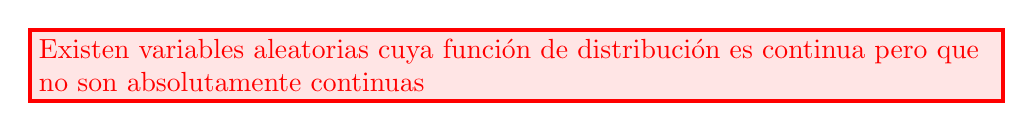
\begin{tikzpicture}
	\node[red, draw=red, fill=red!10, line width=1.5, text width=\textwidth] {Existen \vas cuya función de distribución es continua pero que no son absolutamente continuas};
\end{tikzpicture}

\subsection{Vector aleatorio discreto}
Un vector aleatorio $X$ se dice que es \lb{discreto} si existe un conjunto numerable $\mathcal{S}\in\R^k$ tal que $P(X\in\mathcal{S})=1$.

\lb{Función masa de probabilidad} de una vector aleatorio discreto: \[ P[X=x]=P[X_1=x_1,\dots,X_k=x_k] \]para todo $x=(x_1,\dots,x_k)\in\R^k$, satisfaciendo:
\begin{itemize}[label=$\to$]
\item $P[X=x]\ge0,\;\forall x\in\mathcal{S}$
\item $\sum_{x\in\mathcal{S}}P[X=x]=1$
\end{itemize}
\lb{Función de distribución} de un \vea discreto: \[ F(x)=P[X\le x]= \]

\subsection{Distribuciones marginales}
\subsubsection{Caso continuo}
\begin{itemize}[label=\color{red}\textbullet, leftmargin=*]
	\item \color{lightblue}Distribución marginal de la variable aleatoria $X_i$
\end{itemize}
Sea $X=(X_1,\dots,X_k)$ un \vea continuo con función de densidad $f$ entonces cada componente $X_i$ es de tipo continuo y su función de distribución es; \[ F_{X_i}(x_i)=P[X_i\le x_i]=\int_{-\infty}^{x_i}f_{X_i}(z_i)\mathrm{d}z_i, \]con\[ f_{X_i}=\int_{-\infty}^{+\infty}\cdots\int_{-\infty}^{+\infty}f(z_1,\dots,z_k)\mathrm{d}z_1,\dots, \]

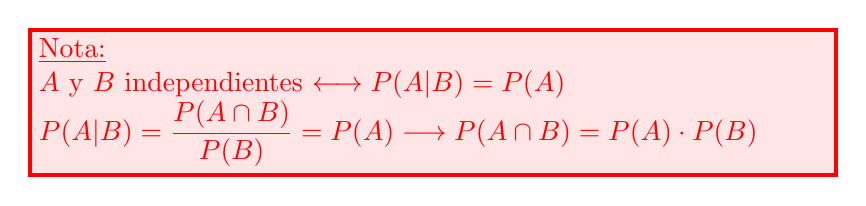
\begin{tikzpicture}
	\node[red, draw=red, fill=red!10, line width=1.5, text width=10cm] {\underline{Nota:}\\
	$A$ y $B$ independientes $\longleftrightarrow P(A|B)=P(A)$\\
	$P(A|B)=\dfrac{P(A\cap B)}{P(B)}=P(A)\longrightarrow P(A\cap B)=P(A)\cdot P(B)$
	};
\end{tikzpicture}

\begin{itemize}[label=\color{red}\textbullet, leftmargin=*]
	\item \color{lightblue}Distribución condicionada al valor de una variable
\end{itemize}

Sea $X=(X_1,\dots,X_k)$

\begin{itemize}[label=\color{red}\textbullet, leftmargin=*]
	\item \color{lightblue}Distribución condicionada a valores de varias variables
\end{itemize}
Sea $X=(X_1,\dots,X_k)$ un vecotr aleatorio continuo

\newpage

\includepdf{"Tareas/Tema 1/Hoja 1"}

\begin{enumerate}[label=\color{red}\arabic*), leftmargin=*]
	\item \lb{Sea $(X,Y)$ un \vea con función de densidad conjunta \[f(x,y)=\begin{cases}
	1 & \text{si }0<x<1,\;0<y<1\\
	0 & \text{en otro caso}
	\end{cases}\] Hallar las distribuciones marginales y condicionadas}
	
	$\underset{0<x<1}{f_X(x)=}\int_{\infty}^{+\infty}f(x,y)\dy=\cancel{\int_{-\infty}^{0}0\dy}+\int_{0}^{1}1\dy+\cancel{\int_{0}^{+\infty}0\dy}=\left[y\right]_{y=0}^{y=1}=1\qquad f_X(x)=\begin{cases}
	1 & \text{si }0<x<1\\
	0 & \text{en otro caso}
	\end{cases}$
	
	$\underset{0<y<1}{f_Y(y)=}\int_{-\infty}^{+\infty}f(x,y)\dx=\int_{0}^{1}1\dx=\left[x\right]_{x=0}^{x=1}=1\qquad f_Y(y)=\begin{cases}
	1 & \text{si }0<y<1\\
	0 & \text{en otro caso}
	\end{cases}$
	
	$f(x,y)=\begin{cases}
	1 & 0<x<1,\;0<y<1\\
	0 & \text{en otro caso}
	\end{cases}$
	
	$\underset{f_X(x^*)>0}{y|x=x^*}\longrightarrow f_{\begin{subarray}{l}
	y|x=x^*\\
	0<x^*<1
	\end{subarray}}=\dfrac{f(x^*,y)}{f_X(x^*)}=\begin{cases}
	1 & 0<y<1\\
	0 & \text{en otro caso}
	\end{cases}$
	
	$f(x,y)=f_X(x)\cdot f_Y(y)$\quad $X$ e $Y$ independientes
	
	\item \lb{Obtener las distribuciones marginales y condicionadas asociadas al vector aleatorio $(X,Y)$ con función de densidad \[ f(x,y)=\begin{cases}
	2 & \text{si }0<x<1,\;0<y<x\\
	0 & \text{en otro caso}
	\end{cases} \]}
	
	$\underset{0<x<1}{f_X(x)=}\int_{-\infty}^{+\infty}f(x,y)\dy=\int_{0}^{x}2\dy=\left[2y\right]_{y=0}^{y=x}=2x\longrightarrow\begin{cases}
	2x & \text{si }0<x<1\\
	0 & \text{en otro caso}
	\end{cases}$
	
	$\underset{0<y<1}{f_Y(y)=}\int_{-\infty}^{+\infty}f(x,y)\dx=\int_{y}^{1}2\dx=[2x]_{x=y}^{x=1}=2-2y\longrightarrow\begin{cases}
	2-2y & \text{si }0<y<1\\
	0 & \text{en otro caso}
	\end{cases}$
	
	Los recintos son dependientes.
	
	$\begin{array}{l}
	y|x=x^*\\
	f_{X}(x^*)>0\\
	\underset{0<x^*<1}{f_{y|x=x^*}}(y|x^*)=\dfrac{f(x^*,y)}{f(x^*)}=\begin{cases}
	\dfrac{2}{2x^*} & 0<y<x^*\\
	0 & \text{en otro caso}
	\end{cases}=\begin{cases}
		\dfrac{1}{x^*} & 0<y<x^*\\
		0 & \text{en otro caso}
		\end{cases}
	\end{array}$
	
	$\begin{array}{l}
	x|y=y^*\\
	f_Y(y^*)>0\\
	\underset{0<y^*<1}{f_{x|y=y^*}}(x|y^*)=\dfrac{f(x,y^*)}{f_Y(y^*)}=\begin{cases}
	\dfrac{2}{2-2y^*} & \text{si } y^*<x<1\\
	0 & \text{en otro caso}
	\end{cases}=\begin{cases}
	\dfrac{1}{1-y^*} & \text{si }y^*<x<1\\
	0 & \text{en otro caso}
	\end{cases}
	\end{array}$
	
	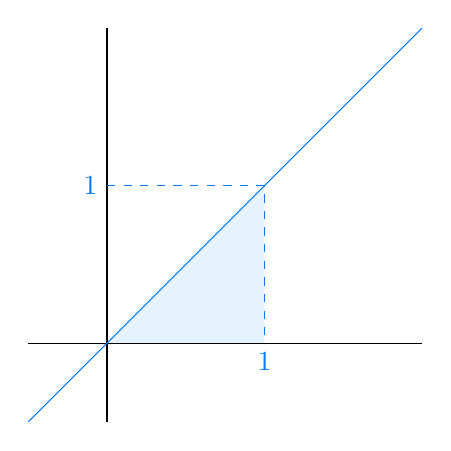
\begin{tikzpicture}[scale=2]
	\fill[lightblue!10] (0,0) -- (1,1) -- (1,0) -- cycle;
	\draw (-0.5,0) -- (2,0);
	\draw (0,-0.5) -- (0,2);
	\draw[lightblue, domain=-0.5:2] plot (\x,\x);
	\draw[lightblue, dashed] (0,1) node[left] {1} -- (1,1) -- (1,0) node[below ] {1};
	\end{tikzpicture}
	
	\item \lb{Sea $(X,Y)$ un \vea con función de densidad \[ f(x,y)=\begin{cases}
	\dfrac{3}{4}\left[xy+\dfrac{x^2}{2}\right] & \text{si }0<x<1,\;0<y<2\\
	0 & \text{en otro caso}
	\end{cases} \]Hallar la distribución marginal de $X$ y la distribución de $Y$ condicionada a $X=\dfrac{1}{2}$.}
	
	
	$\underset{0<x<1}{f_X(x)=}\int_{-\infty}^{+\infty}f(x,y)\dy=\int_{0}^{2}\dfrac{3}{4}\left[xy+\dfrac{x^2}{2}\right]=\dfrac{3}{4}\left[\dfrac{xy^2}{2}+\dfrac{x^2}{2}\cdot y\right]_{y=0}^{y=2}=\dfrac{3}{4}\left(2x+x^2\right)\longrightarrow\begin{cases}
	\dfrac{3}{4}\left(2x+x^2\right) & \text{si }0<x<1\\
	0 & \text{en otro caso}
	\end{cases}$
	
	$\begin{array}{l}
	y|x=x^*\\
	\underset{0<x^*<1}{f_{y|x=x^*}}(y|x^*)=\dfrac{f(x^*,y)}{f(x^*)}=\dfrac{\frac{3}{4}\left(x^*y+\frac{(x^*)^2}{2}\right)}{\frac{3}{4}\left(2x^*+(x^*)^2\right)}=\dfrac{x^*y+\frac{(x^*)^2}{2}}{2x^*+\frac{(x^*)^2}{2}}=\dfrac{x^*y+(x^*)^2}{4x^*+2(x^*)^2}\xrightarrow{x^*=\frac{1}{2}}\dfrac{\frac{1}{2}y+\frac{1}{8}}{2\cdot\frac{1}{2}+\frac{1}{4}}=2\cdot\dfrac{y+\frac{1}{4}}{5}\\
	\begin{cases}
	2\cdot\dfrac{y+\frac{1}{4}}{5} & \text{si }0<y<2\\
	0 & \text{en otro caso}
	\end{cases}
	\end{array}$
	\item \lb{Sea $X=(X_1,X_2)$ un \vea con función masa de probabilidad \[ P[X_1=x_1,X_2=x_2]=\dfrac{k}{2^{x_1+x_2}},x_1,x_2\in\N \]donde $k$ es una constante. Obtener las distribuciones marginales y condicionadas.}
	
	$P[X_1=x_1,X_2=x_2]=\dfrac{k}{2^{x_1+x_2}},\:x_1,x_2\in\N$ (incluido el 0)
	
	$\underset{x_1\in\N}{P[X_1=x_1]}=\sum_{x_2\in \N}\dfrac{k}{2^{x_1+x_2}}=\dfrac{k}{2^{x_1}}\sum_{x_2\in\N}\dfrac{1}{2^{x_2}}=\dfrac{k}{2^{x_1}}\cdot\dfrac{1}{1-\frac{1}{2}}=\dfrac{2k}{2^{x_1}}$
	
	$\underset{x_1^*\in\N}{P[X_2=x_2|X_1=x_1^*]}=\dfrac{P[X_1=x_1^*,X_2=x_2]}{P[X_1=x_1]}=\begin{cases}
	\dfrac{\frac{k}{2^{x_1+x_2}}}{\frac{2k}{2^{x_1}}} = \dfrac{1}{2\cdot 2^{x_2}} & x_2\in\N\\
	0 & \text{en otro caso}
	\end{cases}$
	
	\item \lb{Calcular la función de densidad de una distribución normal bidimensional en $(1,1)$ si las medias son cero, las varianzas 1 y 4, y la covarianza 1.}
	
	Fórmula de la función de densidad de una distribución normal bidimensional: \[ f(x,y)=\dfrac{1}{2\pi\sigma_x\sigma_y\sqrt{1-\rho^2}}\exp\left(-\dfrac{1}{2(1-\rho^2)}\left[\dfrac{(x-\mu_x)^2}{\sigma_x^2}+\dfrac{(y-\mu_y)^2}{\sigma_y^2}-\dfrac{2\rho(x-\mu_x)(y-\mu_y)}{\sigma_x\sigma_y}\right]\right) \]
	
	$\begin{array}{l}
	\mu_x = \mu_y = 0\\
	\sigma^2_x = 1\\
	\sigma^2_y = 4\\
	\rho=\dfrac{\sigma_{xy}}{\sigma_x\cdot\sigma_y}=\dfrac{1}{\sqrt{1}\cdot\sqrt{4}}=\dfrac{1}{2}
	\end{array}\qquad \begin{aligned}
	f(1,1)&=\dfrac{1}{2\pi\cdot1\cdot2\sqrt{1-\left(\frac{1}{2}\right)^2}}\exp\left(-\dfrac{1}{2\left(1-\left(\frac{1}{2}\right)^2\right)}\cdot\left[1^2+\dfrac{1^2}{4}-\dfrac{2\cdot\frac{1}{2}}{1\cdot2}\right]\right)\\
	&=\dfrac{1}{2\pi\sqrt{3}}\exp\left(-\dfrac{2}{3}\cdot\dfrac{3}{4}\right)\\
	&=\dfrac{1}{2\pi\sqrt{3}}\exp\left(-\dfrac{1}{2}\right)\simeq\bboxed{0.0557}
	\end{aligned}$
	\item \lb{Sea $(X,Y)$ un \vea con distribución uniforme en el cuadradado unidad, $[0,1]\times[0,1]$, con función de densidad conjunta \[ f(x,y)=\begin{cases}
	1 & \text{si }0<x<1,\;0<y<1\\
	0 & \text{en otro caso}
	\end{cases} \]Calcular el valor esperado de $g(X,Y)=XY^2$, es decir, $E[XY^2]$.}
	
	
	\item \lb{$(X,Y)$ vector aleatorio discreto con función masa de probabilidad conjunta: \begin{center}
	\begin{tabular}{|c|c|c|}
	\hline
	\backslashbox{X}{Y} & 1 & 2\\ \hline
	1 & $\tfrac{1}{9}$ & $\tfrac{2}{9}$\\
	2 & $\tfrac{2}{9}$ & $\tfrac{4}{9}$ \\ \hline
	\end{tabular}
	\end{center}}
	\begin{enumerate}[label=\color{red}\alph*)]
		\item \db{Calcular $E[X+Y],E[2X+3Y]$.}
		
		
		\item \db{Obtener el vector de medias, la matriz de covarianzas y la matriz de correlaciones del vector $(X,Y)$.}
		
		
		\item \db{¿Son independientes? ¿Están incorreladas?}
		
		
	\end{enumerate}
\end{enumerate}
\end{document}